\section{Branda Gunnarsson}\label{branda-gunnarsson}


\begin{figure}
\centering
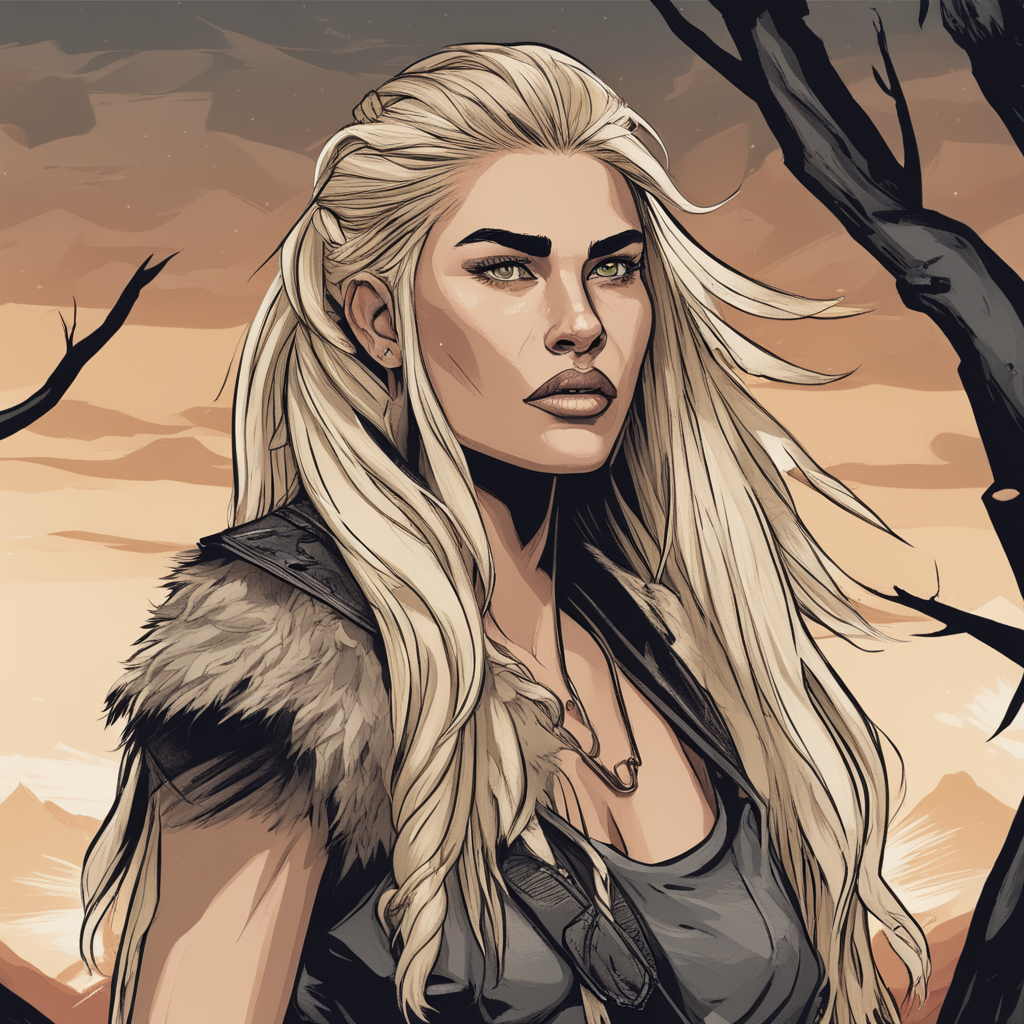
\includegraphics{create-a-digital-illustration-of-branda-a-fierce-and-legendary-woman-with-long-blonde-hair-in-a-hal.png}
\end{figure}

\subsection{Descrizione Generale}\label{descrizione-generale}



Branda Gunnarsson, conosciuta come Branda la Fiera, è una figura
leggendaria che si è guadagnata una fama straordinaria Come feroce
avventuriera sempre alla ricerca di avversari più potenti. La sua forza
titanica, la determinazione inarrestabile e l'impegno senza compromessi
nel proteggere la terra l'hanno resa un'icona indiscussa tra gli
avventurieri delle terre selvagge di Valtara.

\subsection{Biografia}\label{biografia}


\subsubsection{Infanzia}\label{infanzia}


Branda la Fiera è nata nel piccolo villaggio di montagna di
Ducatomarrano, circondato da maestose valli e foreste remote. La sua
infanzia è stata segnata da avventure all'aria aperta e da una profonda
connessione con la natura. Fin da piccola, Branda dimostrava una
straordinaria forza fisica e un amore per la vita all'aria aperta. I
suoi genitori, un abile cacciatore e una maestra tessitrice, le hanno
trasmesso preziose abilità di sopravvivenza.

Tuttavia, il destino ha giocato un brutto scherzo quando, all'età di
otto anni, il suo villaggio fu devastato da una terribile inondazione
causata da una violenta tempesta. Questo evento traumatico ha segnato
profondamente Branda e ha risvegliato in lei una determinazione a
proteggere le persone e la natura.

\subsubsection{Adolescenza}\label{adolescenza}


Dopo l'evento dell'inondazione, Branda ha lasciato il suo villaggio
natale in cerca di avventure. Nell'adolescenza, ha viaggiato per
Valtara, esplorando terre sconosciute e affrontando una serie di sfide.
Si è allenata duramente, affinando le sue abilità nel combattimento e
imparando a sopravvivere nelle condizioni più ostili.

Durante questo periodo, ha incontrato e si è alleata con vari
avventurieri, apprendendo da ognuno di loro e guadagnando una
reputazione per il suo coraggio e la sua abilità nel combattimento. Ha
partecipato a missioni per proteggere carovane, sconfiggere mostri e
assistere le comunità in difficoltà.

\subsubsection{Vita Adulta e giorninostri}\label{vita-adulta-e-giorni-nostri}

Dopo anni di avventure e crescita personale, Branda ha deciso di
stabilirsi nella pericolosa Foresta dei Giganti in cerca di sfide ancora
più grandi. Questa foresta selvaggia e misteriosa è diventata il suo
nuovo territorio di caccia, dove ha combattuto contro molte delle
creature più feroci e rare del mondo. Qui, ha sviluppato ulteriormente
le sue abilità e ha guadagnato una reputazione tra gli avventurieri come
una forza della natura.

Un giorno, mentre era alla ricerca di un leggendario alce d'argento che
infestava la foresta, ebbe una visione straordinaria di uno spirito lupo
della Sila. Questo incontro divino le rivelò la via della redenzione e
la spinta a mettere le sue abilità al servizio della natura e della
pace. Da allora, Branda ha abbandonato la vita errante per unirsi alla
Gilda dei Guardiani Protettori della Sila e dei Lupi, dedicando la sua
forza e il suo coraggio a proteggere la regione di Valtara e a mantenere
l'ordine tra le creature selvatiche e gli abitanti umani

\subsection{Carriera}\label{carriera}


La carriera di Branda la Fiera è segnata da numerosi combattimenti
eroici e imprese leggendarie. La sua fama come avventuriera la precede,
ed è conosciuta per le sue gesta coraggiose nella Foresta dei Giganti,
dove ha affrontato, da sola, creature temibili come gli orsi delle
caverne giganti, i lupi mannari e si dice persino dei troll.

Dopo la sua conversione alla causa della protezione della natura, Branda
ha continuato a dimostrare la sua dedizione, lavorando con la Gilda dei
Guardiani Protettori della Sila e dei Lupi per preservare gli ecosistemi
di Valtara e mantenere la pace tra le creature selvatiche e gli abitanti
umani. La sua forza, abilità nel combattimento e il suo spirito guida le
hanno permesso di diventare una figura rispettata e una guida per i
giovani aspiranti avventurieri.

\subsection{Personalità}\label{personalituxe0}


Branda è conosciuta per la sua personalità forte e sicura di sé. È prona
all'ira quando è necessario, ma ha imparato a canalizzare la sua rabbia
in modo positivo per combattere le minacce che si presentano. È
appassionata della birra e delle sfide di forza, spesso partecipando a
gare di bevute e gare di sollevamento pesi nei luoghi che visita.

Tuttavia, la sua dedizione alla protezione della natura e la sua
connessione con lo spirito guida del lupo della Sila le conferiscono
anche un lato compassionevole e altruista. È pronta a difendere gli
oppressi e a sacrificare tutto per mantenere l'armonia nella Valtara. La
sua personalità complessa la rende una figura affascinante nel mondo di
D\&D, ammirata sia per la sua forza fisica che per il suo spirito
indomito.

